\setAuthor{}
\setRound{lõppvoor}
\setYear{2020}
\setNumber{G 3}
\setDifficulty{3}
\setTopic{TODO}

\prob{Käivitusvool}
\begin{wrapfigure}{r}{0.35\textwidth}
  \vspace{-25pt}
  \begin{center}
  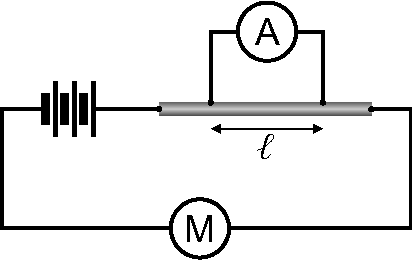
\includegraphics[scale=0.6]{2020-v3g-03-yl.pdf}
  \vspace{-20pt}
  \end{center}
\end{wrapfigure}
Taavet otsustas ära mõõta auto käivitusvoolu tugevuse. Ta leidis ampermeetri
mõõtepiirkonnaga~$I_0=\SI{1}{\milli\ampere}$ ja sisetakistusega~$R_0=\SI{100}{\ohm}$
ja paraja pikkusega jupi vasktoru, mille sisediameeter oli
$d_1=\SI{6}{\milli\meter}$ ja välisdiameeter $d_2=\SI{8}{\milli\meter}$. Ta ühendas
vasktoru jadamisi autoaku ja starteriga (mida võib käsitleda kui takistit) ning ampermeetri rööbiti
vasktoruga nagu kujutatud kõrvaloleval skeemil. Milline tuleks
valida kontaktide vaheline distants~$\ell$, et ampermeetri maksimaalsele
näidule~$I_0$ vastaks mõõdetava voolu suurus $I_1=\SI{500}{\ampere}$?
Vase eritakistus on $\rho=\SI{1.68e-8}{\ohm\meter}$. Ühendusjuhtmete ja
-kontaktide takistused võib lugeda tühiseks.



\hint

\solu
Vasktoru takistus on ilmselt märksa väiksem kui ampermeetri sisetakistus, seega praktiliselt kogu käivitusvool kulgeb läbi vasktoru.

Vasktoru ristlõike pindala (mida vool läbib) on $S=\frac{1}{4}\pi(d_2^2-d_1^2)=\SI{22}{\milli\meter\squared}$. Ühikulise pikkusega torujupi takistus on $R=\rho/S$. Seega voolutugevusel $I_1=\SI{500}{A}$ pingelang vasktoru pikkusühiku kohta
\[
\delta U = RI_1 = \frac{\rho}{S}I_1\approx \SI{0.38}{\volt\per\meter}.
\]
Et läbi ampermeetri tekiks voolutugevus $I_0=\SI{1}{mA}$, on ampermeetrile tarvis rakendada pinge $U=I_0R_0=\SI{0.1}{\volt}$. Selline pingelang moodustub vasktoru pikkusel $\ell=U/\delta U=\SI{0.26}{\meter}$.
\probend